%Introduction

\chapter{1. Introduction}

\section{Persuasive Electric Vehicle}

\subsection{Development History}
\begin{quote}

\end{quote}
\textit{}
\textbf{}

%\thanks{Inspired by Michael Lin}
\marginnote{Inspired by Michael Lin}

\newthought{}

\begin{figure*}[h]
	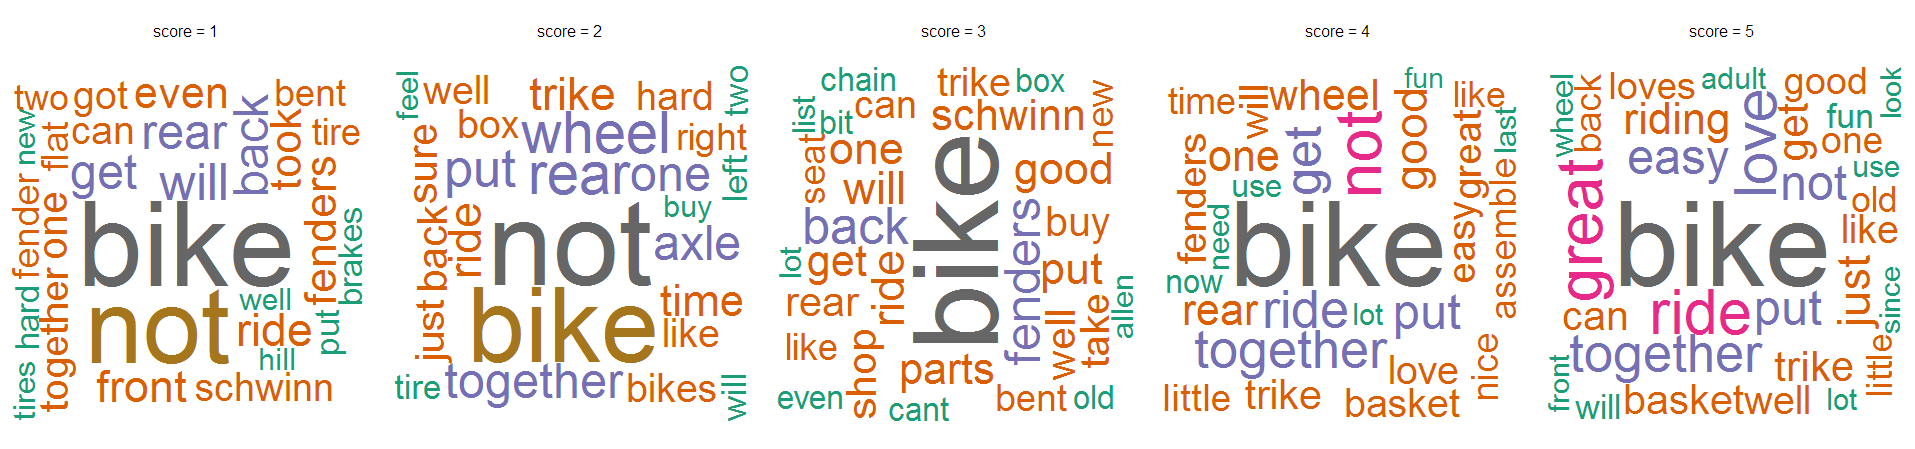
\includegraphics[width=\linewidth]{visuals/Amazon/wordcloud_score_copia}
	\caption{Wordcloud Score}
\end{figure*}

\begin{marginfigure}
	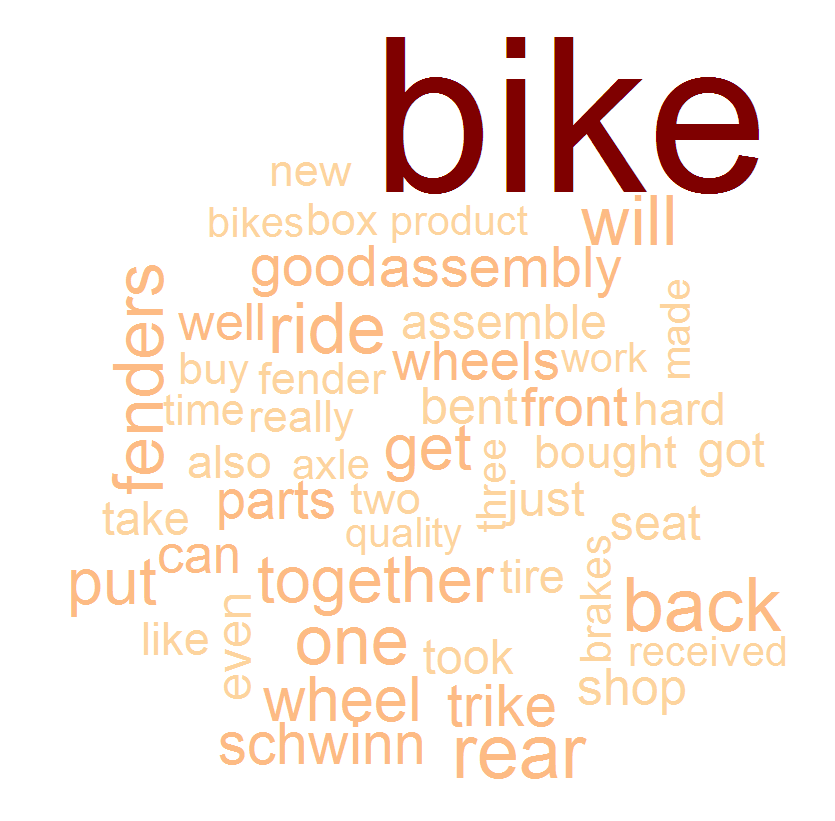
\includegraphics[width=\linewidth]{visuals/Amazon/test.png}
	\caption{Amazon review analysis extracted keywords. 
	Defined by $x=\cos(2\pi z)$, $y=\sin(2\pi z)$}
\end{marginfigure}


\begin{table}%[ht]
  \centering
  \fontfamily{ppl}\selectfont
  \begin{tabular}{ll}
    \toprule
    Margin & Length \\
    \midrule
    Paper width & \unit[8\nicefrac{1}{2}]{inches} \\
    Paper height & \unit[11]{inches} \\
    Textblock width & \unit[6\nicefrac{1}{2}]{inches} \\
    Textblock/sidenote gutter & \unit[\nicefrac{3}{8}]{inches} \\
    Sidenote width & \unit[2]{inches} \\
    \bottomrule
  \end{tabular}
  \caption{Here are the dimensions of the various margins used in the Tufte-handout class.}
  %\label{tab:normaltab}
  %\zsavepos{pos:normaltab}
\end{table}


In 2014,\newline
(1) Prueba 
\cite{Wonham:1614618}
{\small \[ppb = \frac{(we - we_{zero}) - (n*ae - ae_{zero})}{sensitivity}\]}

%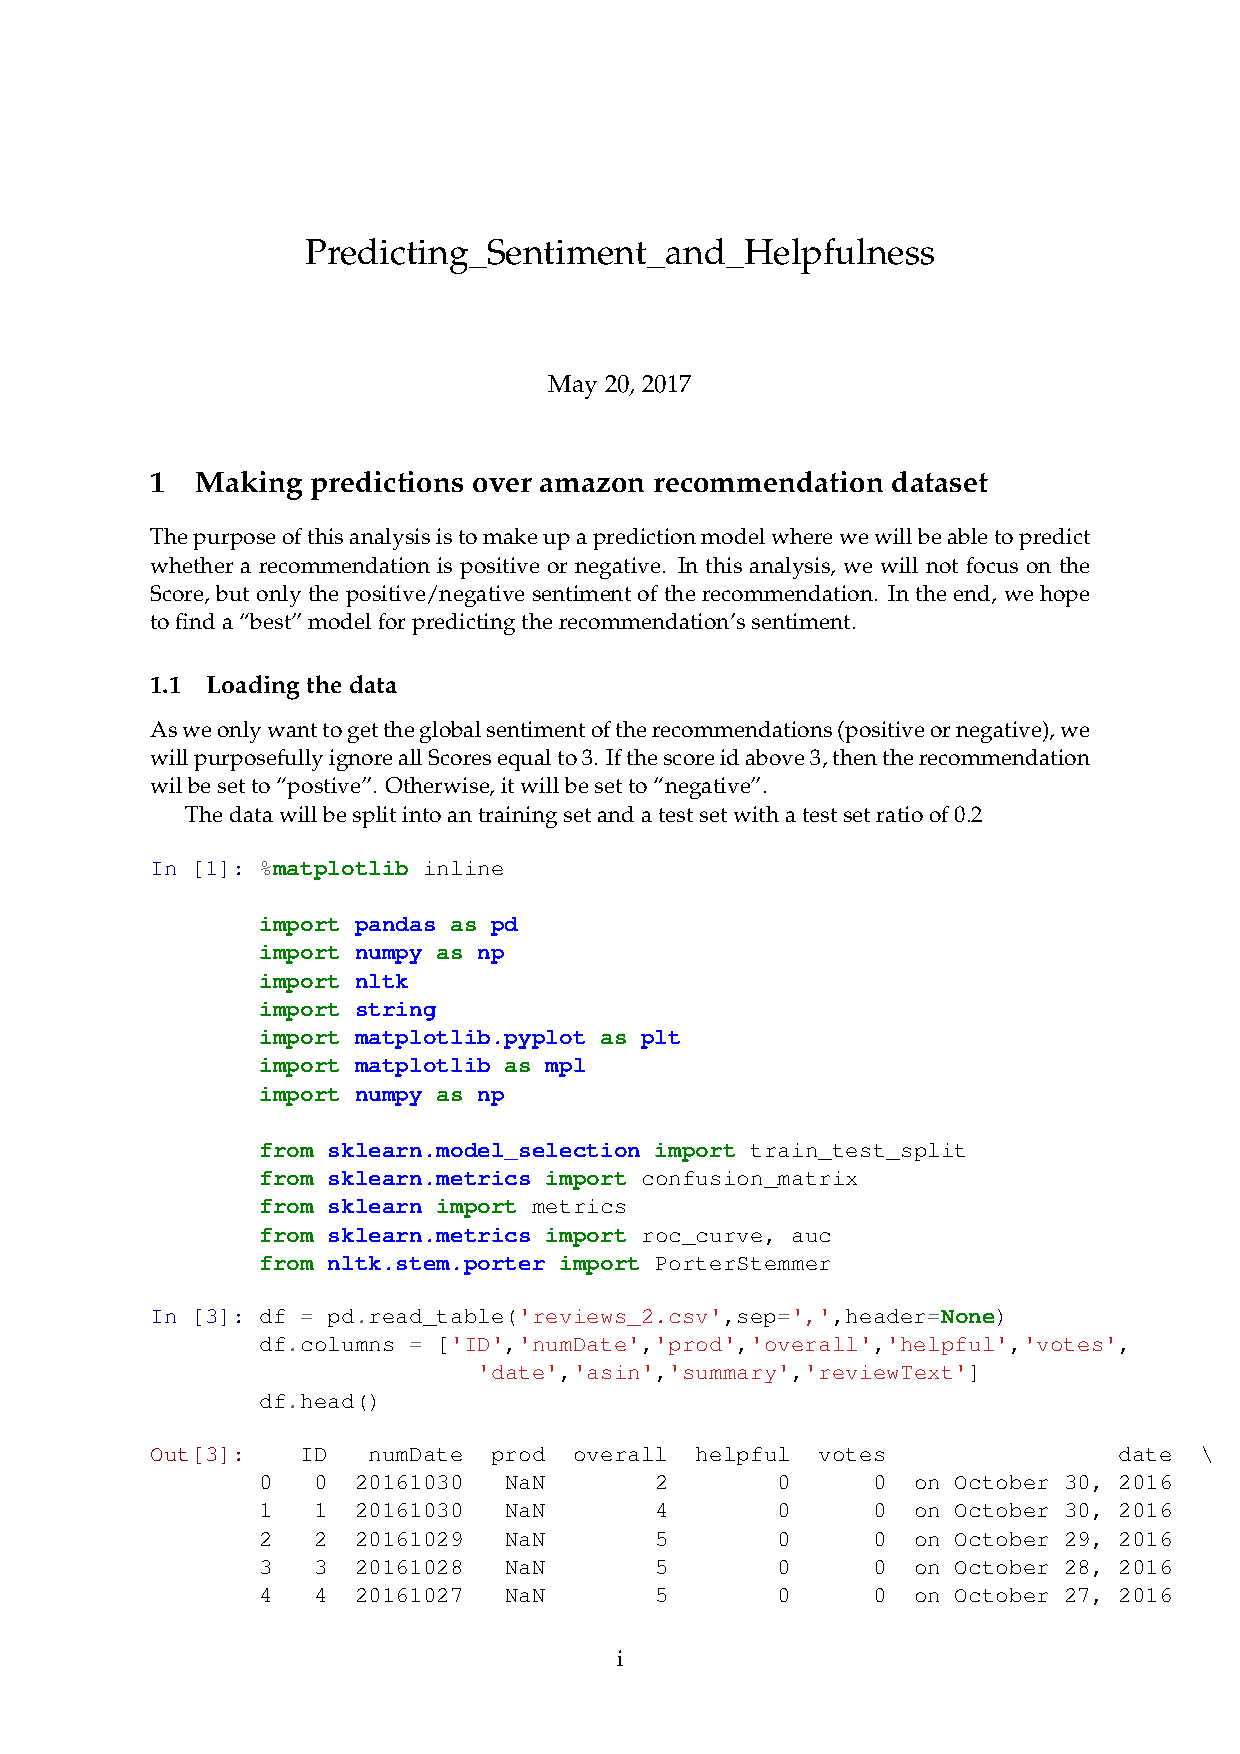
\includepdf[pages=-,scale=1]{pages/Predicting_Sentiment_and_Helpfulness/Predicting_Sentiment_and_Helpfulness.pdf}
%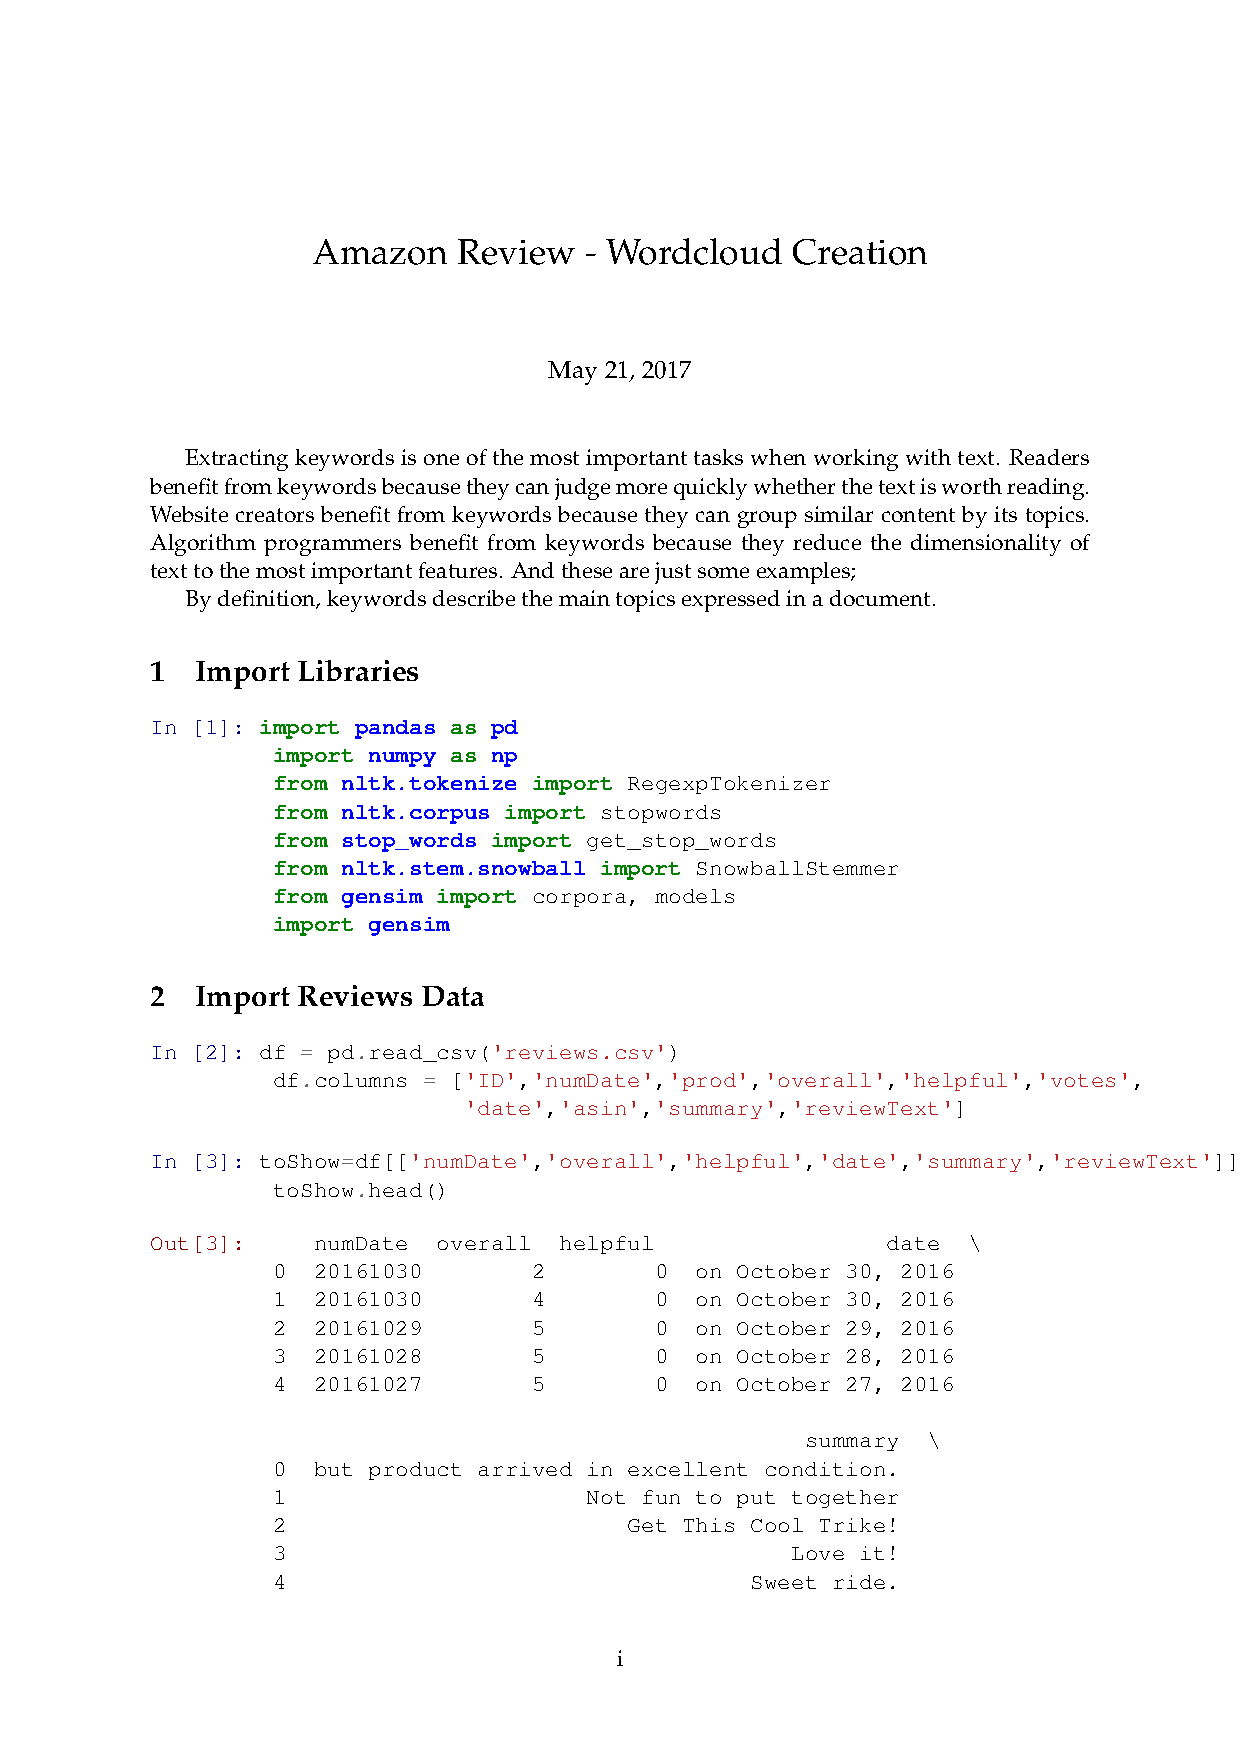
\includepdf[pages=-	,scale=1]{pages/Amazon/Amazon.pdf}

\enlargethispage{10\baselineskip}
\FloatBarrier

%\begin{lstlisting}[style=codedef] ó [style=code] removing @@
%@@Organization@@
%	
%	%\textit{An installation of ChainAPI maintained and curated by an Organization.}%
%
%	@@name@@(string) - the name of the organization.
%	@@url@@(string) - the website URL associated with the organization.
%	@@ch:deployments@@ (related resource) - a collection of deployments associated with the organization.
%	@@ch:contacts@@ (related resource) - a collection of contacts associated with the organization.
%
%\end{lstlisting}

%\begin{figure}[htb]
% 	\includegraphics[width=\textwidth + \marginparwidth]{schematics/la_schematic6}               
%\end{figure}

%here's text referencing the (Table \ref{tab:sample_table}).
%
%\begin{table}
%  \centering
%  \begin{tabular}{l l l l l}
%    Column A & Column B & Column C & Column D & Column E \\
%    \toprule
%    A & B & C & D & E
%  \end{tabular}
%  \caption{A meaningless table}
%  \label{tab:sample_table}
%\end{table}

%\begin{marginfigure}[3.5cm
% 	\includegraphics[width=\textwidth]{visuals/learnairV1}               
% 	 \caption{LearnAir Sensor installed at MassDEP site, opened}
%  	\label{fig:learnairv1}
%\end{marginfigure}
%
%\begin{figure}[htb]
% 	\includegraphics[width=\textwidth]{visuals/learnairV1_labeled}               
% 	 \caption{LearnAir Sensor installed at MassDEP site}
%  	\label{fig:learnairv1_labeled}
%\end{figure}